\chapter{Problem analysis}

In this chapter, we formalize the concept of planning to help us with formally introducing the studied transportation problems. We will also briefly discuss specifics of the Transport domain and mention similar studied problems.

\section{Automated planning}

Planning is usually defined as the reasoning side of acting -- an abstract deliberation
process that chooses and organizes actions by anticipating their outcomes. \citep[Section~1.1]{Ghallab2004}
It seems only natural that we want to have computers to do this strenuous activity for us.
Automated planning is an attempt at just that -- it is an area of Artificial Intelligence (AI) that
studies the planning process computationally. \citep[Section~1.1]{Ghallab2004}

Unfortunately, the specific situations in which we want to use automated planning are very diverse --
from devising a sequence of actions to shut down a nuclear power plant to planning the robotic arm
movements in an assembly line or devising the complex motor activations for space aircraft positioning.
Due to this, people are often interested in domain-independent planning, where the planner gets information
about both the domain and the specific problem and attempts to devise a plan using only the provided knowledge
and the planner's previously built-in processes. \citep[Section~1.3]{Ghallab2004}

On the other hand, domain-specific planning, where domain knowledge has been built into the planner,
has obvious advantages when solving problems in that domain -- all the while being useless on problems of other
domains. \citep[Section~1.3]{Ghallab2004}

\subsection{Planning model}

As a basis for the later-defined representation of planning, we first define
a conceptual model similar to the restricted model in \citep[Section~1.4, Section~1.5]{Ghallab2004}.

\begin{defn}[State-transition system]\label{defn:state-transition-sys}
A (restricted) state-transition system is a 3-tuple $\Sigma = (S, A, \gamma)$, where:
\begin{itemize}
\item $S = \{s_1, s_2, \ldots\}$ is a finite and fully observable set of states,
\item $A = \{\noop, a_1, a_2, \ldots\}$ is a finite set of actions;
\item $\gamma: S \times A \to S \cup \{\emptyset\}$ is a state-transition function,
where $\forall s \in S : \gamma(s, \noop) = s$,
and $\forall s \in S\,\exists a \in A : \gamma(s, a) \neq \emptyset$; and
\item $\Sigma$ is static and offline,
it only changes when an action is applied to it and does not change while planning.
\end{itemize}
In the basic version, all actions have no duration.
\end{defn}

State transition systems approximately correspond to what we will refer to as \textit{planning domains}.
They define which states and which actions we work with and how they
are related, but they do not state anything about objectives, or what
we want to achieve with planning.

Given a state transition system $\Sigma$, planning aims to find which
sequence of actions to apply to which states in order to achieve some objective.
The objective can be defined in various ways -- we might want the planner
to devise a plan that
does not enter specific states, or contrary to that, visits each of a set of states,
or just end at a chosen state.
We will use the last choice to formalize the notion of a \textit{planning problem}.

\begin{defn}[Planning problem]\label{defn:planning-problem}\citep[Part~I]{Ghallab2004}
A planning problem is a 5-tuple $\mathcal{P} = (S, A, \gamma, s_0, g)$, where:
\begin{itemize}
\item $(S, A, \gamma)$ is a state-transition system;
\item $s_0 \in S$ is an initial state; and
\item $g \subseteq S$ is a set of goal states.
\end{itemize}
\end{defn}

Now that we have defined a \textit{planning problem} we can specify what we meant
by the planner generating a sequence of actions to achieve a goal -- we will
call this sequence a \textit{plan}.
For notation purposes, we define $[k] := \{1, 2, \ldots, k\}$ for all $k \in \N$

\begin{defn}[Plan]\label{defn:plan}\citep[Section~1.5]{Ghallab2004}
For a planning problem $\mathcal{P} = (S, A, \gamma, s_0, g)$,
a plan is a finite ($k \in \N$) sequence of actions $(a_1, a_2, \ldots, a_k)$ where
$\forall i \in [k] : a_i \in A$ such that
$\forall i \in [k] : \gamma(s_{i-1}, a_i) = s_i$ and $s_k \in g$.
\end{defn}

\noindent A basic planning model (see Figure~\ref{fig:planning-model}) consists of three components:

\begin{itemize}
\item A \textit{state-transition system} $\Sigma$ that evolves by its state-transition function using the actions
it receives.
\item A \textit{controller} -- given an input state $s \in S$ provides an action $a \in A$ as output according
to a plan.
\item A \textit{planner} -- uses a description of $\Sigma$ to synthesize a plan for the controller
to execute in order to achieve the objective.
\end{itemize}

\begin{figure}[htb]
\begin{center}
\includegraphics[width=0.7\textwidth]{../imga/planning_model}
\end{center}
\caption{Typical planning model for offline planning. Adapted from \citep[Figure~1.3]{Ghallab2004}.}
\label{fig:planning-model}
\end{figure}

\subsection{Classical planning}\label{classical-planning}

Although the previously defined restricted state-transition system is a simplification of real-world
domains, it is a useful one. 
This simplification has historically been studied as classical planning.
There are several theoretical domain-independent representations
of planning problems in classical planning. \citep[Chapter~2]{Ghallab2004}

\subsubsection{Set-theoretic representation}

Leveraging propositional logic, both the planning domain and problem
are represented with the notion
of proposition symbols $L = \{p_1, p_2, \ldots\}$.
Each state is defined as a subset of propositions of $L$ -- those propositions
which hold in the given state. $S$ is closed under the application of each
action $a \in A$.

An action $a$
is a triple of sets of propositions of $L$.
We denote the sets $a = (\precond(a), \effects^-(a), \effects^+(a))$, where:
\begin{itemize}
\item $\precond(a)$ are the \textit{preconditions} of an action: the set of
propositions that must hold in the current state for the action to be applicable to it;
\item $\effects^-(a)$ are the \textit{negative effects} of an action:
the set of propositions
that will no longer hold in the state once the action is applied; and
\item similarly, $\effects^+(a)$ are the \textit{positive effects} of an action:
the set of propositions that will be true in the state once the action is applied.
\end{itemize}

The state-transition function is $\gamma(s, a) = (s - \effects^-(a)) \,\cup\,
\effects^+(a)$ if $a$ is applicable to $s$,
otherwise $\gamma(s, a)$ is undefined. Goal states $S_g$ are defined as
$S_g = \{s \in S \,|\, g \subseteq s\}$, where
$g \subseteq L$ is any chosen set of propositions. The propositions $g$ are called
\textit{goal propositions}.

\subsubsection{Classical representation}

The classical representation generalizes the set-theoretic representation using first-order logic,
without functions.
States are sets of ground atoms of a first-order language.
Actions are ground instances of \textit{planning operators},
triples $o = (\name(o), \precond(o), \effects(o))$:

\begin{itemize}
\item $\name(o)$ is a syntactic expression of the given operator;
\item $\precond(o)$ and $\effects(o)$ are sets of literals
(atoms and their negations), similar in use to their equivalents
in the set-theoretic case.
\end{itemize}

The definition of the state-transition function also stays the same.
Goal states are defined as the set of states that satisfy $g$,
the \textit{goal}, where $g$ is any set of ground literals.

Both the set-theoretic and the classical representations follow the \textit{Closed world assumption} -- that any atom/predicate not present in the state does not hold in the state.

\subsubsection{State-variable representation}

The state-variable representation substitutes the use of relations of the previous
representation for functions,
using the concept of state variables. State variables are functions
that take the state as an input and serve as characteristic attributes, defining the state. We usually use a more practical way of defining these functions -- we assume
the current state as an input without denoting it, and instead add different inputs.

For example, a useful set of state-variable functions for a domain that contains a road
network and vehicles might be: $$\mathrm{location}_{v}: S \to \mathrm{locations},$$
where $v \in \mathrm{vehicles}$.
Instead, we could define a single function:
$$\mathrm{location'}: \mathrm{vehicles} \times S \to \mathrm{locations},$$
and afterwards 
$$\mathrm{location''}: \mathrm{vehicles} \to \mathrm{locations},$$
using $\mathrm{location''}(v) = \mathrm{location'}(v, state_{cur})$, where $state_{cur}$ is the current state.

Planning operators are defined similarly to the classical representations, but
$\precond(o)$ is now a set of expressions on state variables and relations.
Also, $\effects(o)$ is defined as a set of assignments of values to state variables.
The state transition function is defined analogously: an action $a$ (ground instance
of operator $o$)
is applicable to a state $s$ if the $\precond(o)$ condition is true given the values
of state variables in state $s$. The effects of the action change the state variables
according to the assignments in $\effects(o)$ and the corresponding values of state
variables in state $s$, implicitly transitioning to a different state.
The goal is defined as a set of ground state variables and their corresponding values.
\citep[Section~2.5.2]{Ghallab2004}

\subsubsection{Extensions of representations}

We will later extend these representations using types.
To see how types fit into our previously defined representations, we can
define a \textit{type} as a unary predicate, which has the value true
if and only if the predicate's argument is of the given type.
We can then add these predicates as preconditions of actions.
Adding types will make the domain and problem formulations
easier to read and gives additional information
to planners, making them more efficient.
\citep[Section 2.4.1]{Ghallab2004}

\subsubsection{State-space planning and Plan-space planning}

\TODO{add definitions and examples}

\subsubsection{Neoclassical planning}

Neoclassical planning uses largely the same theoretical foundations as classical 
planning. What is different is the approach to planning using those foundations
-- instead of search space nodes being a sequence of actions or a partially ordered
set of actions, we view them as a set of several partial plans.
\citep[Part~II]{Ghallab2004}

The most famous result in neoclassical planning is Blum's and Furst's the GraphPlan algorithm. \citep{Blum1997}
It is out of the scope of this text to describe it in detail
(see \citep[Section~6.3]{Ghallab2004}).
GraphPlan makes heavy use of a data structure called a \textit{planning graph},
which caused a breakthrough in the field of planning -- bigger problems could
now be practically solved.

\TODO{consider describing planning graphs}

\subsubsection{Temporal planning}

\TODO{temporal planning \citep[Chapter~14]{Ghallab2004}, possibly \citep[Chapter~15]{Ghallab2004}, small reference to the temporal Transport domain variant}.



\subsection{Planning in practice}

In practice, many assumptions we made get violated and many additional requirements arise
due to various business or social requirements. They allow us, however, to work
on problems that are more general and can therefore be applied to multiple scenarios.
Businesses can often add minor tweaks on top of the obtained results so that
their needs are satisfied. 
For example, online planning can often be foregone for some form of \textit{windowed} planning,
where we plan a certain time window offline and move on to the next window,
repeating the process regularly.

Planners, in practice, are computer programs that are fed two files as input
-- the domain file and the problem file. After that, they proceed with their internal calculations
and upon finishing (or not) return a plan (or not). 
We can then evaluate that plan, see if it meets our criteria and, potentially,
execute it in the real world.

What we are missing from a bare plan is the allocation of specific resources.
Scheduling addresses the problem of how to perform a given set of actions (a plan)
using a limited number of resources in a limited amount of time and
this is crucial to practical usage of any such plan. \citep[Chapter~15]{Ghallab2004}

In this text, we will only study the abstracted and simplified first part of this whole process
-- finding the ``best'' actions that lead to a specified goal.




\section{Transport domain description}

Transport is a planning domain designed for
the International Planning
Competition\footnote{\url{http://www.icaps-conference.org/index.php/Main/Competitions}}
(IPC), which is part of the International Conference on Automated Planning and
Scheduling\footnote{\url{http://www.icaps-conference.org/index.php/Main/HomePage}} (ICAPS).

Originally, Transport appeared at 
IPC-6\footnote{\url{http://icaps-conference.org/ipc2008/deterministic/Domains.html}} which took place in 2008.
Since then, it has been used in two IPCs,
specifically IPC-7\footnote{\url{http://www.plg.inf.uc3m.es/ipc2011-deterministic/}} in 2011
and IPC-8\footnote{\url{https://helios.hud.ac.uk/scommv/IPC-14/}} in 2014.

There are a few basic formulations of the Transport domain family (i.e.~``similar Transport domains'').

\subsection{Common traits of Transport domains}

Transport is a logistics domain -- vehicles drive around on a (generally asymmetric) positively-weighted oriented graph, picking up and dropping packages along the way.
All vehicles have limited capacities (the sum of package sizes they can carry).
Picking up or dropping a package costs 1 unit. The cost of driving along a road is equal to the edge weight
(in other words, the road length).
The general goal is to minimize the total cost
while delivering all packages to their destination. A few Transport problems
also request that the trucks be positioned at certain locations in the graph
after finishing their deliveries.

\subsection{Transport STRIPS}\label{transport-strips}

STRIPS, the Stanford Research Institute Problem Solver,
was a planner proposed in the 1970's by \citet{Fikes1971}.
The influence of STRIPS was, however, not due to the planner,
but the language used to describe its inputs -- the planning operators and goals.
That is why we sometimes refer to classical planning (Section~\ref{classical-planning})
as STRIPS planning. For the purposes of this text, we will use these terms interchangeably.

In the STRIPS variant of the Transport domain,
all packages have a size of 1 and vehicles can drive around infinitely,
only incurring the cost of the travel. This being a classical STRIPS domain,
it does not assume time in any sense,
so actions have no duration and are applied one after the other, sequentially.

This formulation contains three basic planning operators:

\begin{itemize}
\item \verb+drive+: where a vehicle drives to an adjacent location
along a road that is connected to its current location;
\item \verb+pick-up+: where a vehicle that is stationary at a location picks up a co-located package; and
\item \verb+drop+: where a stationary vehicle drops a package off at its location.
\end{itemize}

In all the datasets, this domain variant is denoted as \textit{Transport sequential}
or \textit{transport-strips} and we will alternate between these terms in this text.

\subsection{Transport Numeric}\label{transport-numeric}

The numeric variant adds the concept of fuel on top of the STRIPS variant.
All roads have an additional cost, called \verb+fuel-demand+, which is
subtracted from a vehicle's \verb+fuel-left+ value if it chooses to drive along that road.
Additionally, all vehicles have a maximum fuel capacity \verb+fuel-max+,
which they regain upon being the target of a \verb+refuel+ action. This action can only
be executed at a location that is marked as having a petrol station. Petrol stations
are static with respect to a given planning problem instance.

This variant is usually denoted as \textit{Transport numeric} or \textit{transport-numeric}.

\subsection{Transport Temporal}\label{transport-temporal}

The temporal Transport domain is usually denoted as \textit{Transport temporal} or, confusingly,
also \textit{transport-numeric}. A major difference with respect to the numeric variant is
the addition of time. All actions now have a duration (\verb+pick-up+ and \verb+drop+ both have a
duration of 1, \verb+refuel+ has a duration of 10, and the duration of \verb+drive+ is
equal to the length of the road we are driving along). Furthermore, packages can now have any integral size.

The addition of time poses numerous technical complications when formalizing this variant
-- its PDDL formulation significantly differs the two previous ones, but only in technical details.
One important technicality is that a vehicle cannot pick up or drop packages concurrently -- it always handles packages one at a time. Also, vehicles cannot do other actions during driving to another location (they are essentially placed ``off the graph'' for the duration of driving).

The overall goal remains largely the same (deliver packages to their destinations), but we no longer optimize the total cost. Instead, we now minimize the total duration of a plan (in practice, this translates to minimizing
maximum end time over all actions).



\section{Transport domain formulation}

We will now translate the informal description of the Transport domain from the previous section to the formal representations we defined in Section~\ref{classical-planning}. We will not formulate all the domain variants in all representations as
they are very much alike and not needed for the comprehension of the following chapters.

\subsection{Transport's classical representation}\label{transport-classical-representation}

We are now able to show the sequential Transport domain in one of the representations
previously defined, namely,
the classical representation (Figure~\ref{code:classical-strips}).
Note that this representations does not contain the notion of a \textit{total cost}
of a plan that we will optimize for later.
The predicates used are:

\begin{itemize}
\item \verb+at(o, l)+: the package or vehicle \verb+o+ is at the
location \verb+l+;
\item \verb+capacity(v, s)+: the vehicle \verb+v+ currently has \verb+s+ free space -- \verb+s+ is a variable for space literals, a set of literals denoting the amount of space (essentially interpretable as a finite set of integers);
\item \verb+capacity-predecessor(s1, s2)+: the space literal represented by \verb+s1+
is directly smaller than the literal represented by \verb+s2+;
\item \verb+in(p, v)+: the package \verb+p+ is in the vehicle \verb+v+; and
\item \verb+road(l1, l2)+: the location \verb+l1+ is directly adjacent to the location
\verb+l2+ by a road.
\end{itemize}

\begin{figure}[htb]
\begin{code}
drive(v, l1, l2)
  ;; vehicle v moves from location l1 to an adjacent location l2
  precond: at(v, l1), road(l1, l2)
  effects: not at(v, l1), at(v, l2)

pick-up(v, l, p, s1, s2)
  ;; vehicle v picks up package p at location l,
  ;; decreasing its capacity from s2 to s1
  precond: at(v, l), at(p, l), capacity-predecessor(s1, s2),
           capacity(v, s2)
  effects: not at(p, l), in(p, v), capacity(v, s1),
           not capacity(v, s2)
  
drop(v, l, p, s1, s2)
  ;; vehicle v drops package p at location l,
  ;; increasing its capacity from s1 to s2
  precond: at(v, l), in(p, v), capacity-predecessor(s1, s2),
           capacity(v, s1)
  effects: not in(p, v), at(p, l), capacity(v, s2),
           not capacity(v, s1)
\end{code}
\caption{Classical formulation of \texttt{transport-strips}.}
\label{code:classical-strips}
\end{figure}

The numeric variant  adds the \verb+refuel+ operator, changes the \verb+drive+
operator, and adds a new fuel-related predicate \verb+has-petrol-station(l)+, that is true when the given location \verb+l+ has
a petrol station.
To model fuel, we need the addition of a few functions, namely:

\begin{itemize}
\item \verb+fuel-demand(l1, l2)+: the amount of fuel needed to drive
from location \verb+l1+ to location \verb+l2+;
\item \verb+fuel-left(v)+: the amount of fuel left in
the vehicle \verb+v+; and
\item \verb+fuel-max(v)+: the maximum amount of fuel
the vehicle \verb+v+ can contain, i.e. its fuel tank capacity.
\end{itemize}

It is obvious that we could substitute the functions for relations
and a finite amount of literals for any given problem instance of
the domain in this representation,
so that it adheres to the definition of a classical formulation.
\TODO{proof?}

We also abuse the notation with \verb+decrease+ and \verb+assign+;
the left parameter's value is to be decreased by the right
parameter's value or the left parameter's value is to be overridden
by the right parameter's value, respectively.

See Figure~\ref{code:classical-numeric} for exact differences
in the representation after adding fuel.

\begin{figure}[htb]
\begin{code}
drive(v, l1, l2)
  ;; vehicle v moves from location l1 to an adjacent location l2
  precond: at(v, l1), road(l1, l2), fuel-left(v) >= fuel-demand(l1, l2)
  effects: not at(v, l1), at(v, l2),
           decrease(fuel-left(v),  fuel-demand(l1, l2))
  
refuel(v, l)
  ;; vehicle v is refueled to the maximum at location l
  precond: at(v, l), has-petrol-station(l)
  effects: assign(fuel-left(v), fuel-max(v))
\end{code}
\caption{Classical formulation of \texttt{transport-numeric}'s differences.}
\label{code:classical-numeric}
\end{figure}

\subsection{Temporal Transport's classical representation}

\TODO{code + explanation}

\subsection{Transport's state-variable representation}

We are now also able to show the sequential Transport domain
in the state-variable representation (Figure~\ref{code:statevar-strips}).
Some predicates (\verb+at+, \verb+capacity+ and \verb+in+) have been transformed
into state-variable functions with largely the same semantics as in
Section~\ref{transport-classical-representation}. Again, we leave out
the \textit{total cost} notion.

\begin{figure}[htb]
\begin{code}
drive(v, l1, l2)
  ;; vehicle v moves from location l1 to an adjacent location l2
  precond: at(v) = l1, road(l1, l2)
  effects: at(v) <- l2

pick-up(v, l, p, s1, s2)
  ;; vehicle v picks up package p at location l,
  ;; decreasing its capacity from s2 to s1
  precond: at(v) = l, at(p) = l, capacity-predecessor(s1, s2),
           capacity(v) = s2
  effects: at(p) <- nil, in(p) <- v, capacity(v) <- s1
  
drop(v, l, p, s1, s2)
  ;; vehicle v drops package p at location l,
  ;; increasing its capacity from s1 to s2
  precond: at(v) = l, in(p) = v, capacity-predecessor(s1, s2),
           capacity(v) = s1
  effects: in(p) <- nil, at(p) <- l, capacity(v) <- s2
\end{code}
\caption{State-variable formulation of \texttt{transport-strips}.}
\label{code:statevar-strips}
\end{figure}

The numeric variant again adds the \verb+refuel+ operator along with
a few fuel-related state-variable functions and predicates, and changes 
the \verb+drive+ operator (Figure~\ref{code:statevar-numeric}).

\begin{figure}[htb]
\begin{code}
drive(v, l1, l2)
  ;; vehicle v moves from location l1 to an adjacent location l2
  precond: at(v) = l1, road(l1, l2), fuel-left(v) >= fuel-demand(l1,l2)
  effects: at(v) <- l2, fuel-left(v) <-  fuel-demand(l1, l2)
  
refuel(v, l)
  ;; vehicle v is refueled to the maximum at location l
  precond: at(v) = l, has-petrol-station(l)
  effects: fuel-left(v) <- fuel-max(v)
\end{code}
\caption{State-variable formulation of \texttt{transport-numeric}'s differences.}
\label{code:statevar-numeric}
\end{figure}

\subsection{PDDL}\label{pddl}

Originally proposed by McDermott et al. in 1998 for the 1$^{\mathrm{st}}$ International Planning
Competition\footnote{\url{http://ipc98.icaps-conference.org/}},
the Planning Domain Definition Language\citep{McDermott1998} (PDDL) has become
a de facto standard language for modelling planning domains and problems,
continually evolving to the needs of the
research community and the needs of the IPC itself in the future years.

PDDL was inspired by the language used to describe STRIPS\citep{Fikes1971}
and the numerous languages that sparked from it.
It has a Lisp-like\footnote{\url{https://en.wikipedia.org/wiki/Lisp_(programming_language)}}
declarative syntax and is very extensible.
Not many planners support PDDL in its entirety -- they usually support 
several ``feature subsets'', called \textit{requirements}.
Over time, PDDL has evolved from the originally proposed version 1.2
to the now standard version 3.1. Several extensions and successors were proposed,
like Multi-Agent PDDL\comment{\footnote{\url{http://agents.fel.cvut.cz/codmap/}}}
(MA-PDDL) and
Probabilistic PDDL\comment{\footnote{\url{http://www.tempastic.org/papers/CMU-CS-04-167.pdf}}}
(PPDDL).

All formulations of the Transport domain use the basic PDDL version, with the requirement \verb+typing+.
The STRIPS variant additionally needs \verb+action-costs+, while the numeric variant
requires \verb+numeric-fluents+ and \verb+goal-utilities+.
The temporal domain is similar in requirements to the numeric one, except for
substituting \verb+goal-utilities+ for \verb+durative-actions+.
One problem with the diversity of these domain formulations is that rarely does
a single planner support the union of all these requirements.
We show the capabilities of individual studied planners
later on, in Table~\ref{tab:plannner-requirements-comparison}.

For reference, we show the PDDL representation of the sequential variant of
the Transport domain in Figure~\ref{code:pddl-strips}.

\begin{figure}[htb]
\begin{code}
(define (domain transport)
  (:requirements :typing :action-costs)
  (:types
        location target locatable - object
        vehicle package - locatable
        capacity-number - object)
  (:predicates 
     (road ?l1 ?l2 - location)
     (at ?x - locatable ?v - location)
     (in ?x - package ?v - vehicle)
     (capacity ?v - vehicle ?s1 - capacity-number)
     (capacity-predecessor ?s1 ?s2 - capacity-number))
  (:functions
     (road-length ?l1 ?l2 - location) - number
     (total-cost) - number)
     
  (:action drive
    :parameters (?v - vehicle ?l1 ?l2 - location)
    :precondition (and (at ?v ?l1) (road ?l1 ?l2))
    :effect (and (not (at ?v ?l1)) (at ?v ?l2)
        (increase (total-cost) (road-length ?l1 ?l2))))
        
 (:action pick-up
    :parameters (?v - vehicle ?l - location ?p - package
                 ?s1 ?s2 - capacity-number)
    :precondition (and (at ?v ?l) (at ?p ?l)
        (capacity-predecessor ?s1 ?s2) (capacity ?v ?s2))
    :effect (and (not (at ?p ?l)) (in ?p ?v) (capacity ?v ?s1)
        (not (capacity ?v ?s2)) (increase (total-cost) 1)))
        
  (:action drop
    :parameters (?v - vehicle ?l - location ?p - package
                 ?s1 ?s2 - capacity-number)
    :precondition (and (at ?v ?l) (in ?p ?v)
        (capacity-predecessor ?s1 ?s2) (capacity ?v ?s1))
    :effect (and (not (in ?p ?v)) (at ?p ?l) (capacity ?v ?s2)
        (not (capacity ?v ?s1)) (increase (total-cost) 1))))
\end{code}
\caption{PDDL formulation of \texttt{transport-strips}.}
\label{code:pddl-strips}
\end{figure}





\section{The Vehicle Routing Problem}

\TODO{mention Dantzig} \citep{Dantzig1959}

\TODO{mention Braekers} \citep{Braekers2016}

\TODO{mention Montoya} \citep{Montoya-Torres2015}

\TODO{mention Neo} \citep{ResearchGroup2013}

\subsection{Constraint Satisfaction Problems}

\subsection{Problem formulation}

\subsection{Comparison to the Transport domain formulation}

\subsection{Formulating the sequential Transport domain as a VRP problem}

\TODO{Ghallab 8.3}
